\chapter{The \lhcb\ experiment}
\label{chap:intro:lhcb}

The \lhcb\ experiment comprises a collaboration of around one thousand 
scientists and engineers, and a particle detector situated at point 8 of the 
\cern\ \ac{LHC}.
The general goal of the experiment is to explore the area of \emph{heavy 
  flavour physics}, that is the interactions of charm and beauty quarks and 
particles that contain them.
Specific aims will be given in \cref{chap:intro:lhcb:physics}, and the design 
and construction of the detector will be described in 
\cref{chap:intro:lhcb:detector}.
First, a brief introduction to the mechanisms of a high-energy particle physics 
experiment will be given, such that the particular requirements of a heavy 
flavour experiment can be related to the design of a detector.

Heavy flavour hadrons, such as the \PBs meson, have short lifetimes, and do not 
fly far enough to interact with active elements of a detector before decaying.
By the studying the properties of decay products with longer lifetimes, the 
properties of the unseen heavy flavour hadrons can be inferred, to be compared 
with those predicted by the \ac{SM}.
% Such properties include production and decay rates, lifetimes, and masses.

The momentum four-vector $\fvec{p}$ of a particle is defined by three spatial 
components, equal to components of the momentum three-vector $\vec{p}$, and the 
energy $E$
\begin{equation}
  \fvec{p} = \begin{pmatrix}E\\\vec{p}\end{pmatrix}
           = \begin{pmatrix}E\\p_{x}\\p_{y}\\p_{z}\end{pmatrix}.
  \label{intro:lhcb:four_momentum}
\end{equation}
Both the energy and the momentum can be measured, using techniques which will 
be discussed later.
The mass of every massive particle is unique, and so by knowing the 
four-momentum of a particle, one implicitly knows its identity by knowing the 
mass using the relation
% The energy can either be measured directly, using methods discussed later, or 
% computed using an assumed mass \mass\ and the magnitude of the measured 
% momentum three-vector $\ptot = |\vec{p}|$
\begin{equation}
  E = \sqrt{p^{2} + m^{2}}.
  \label{intro:lhcb:energy}
\end{equation}
To compute the four-momentum of a heavy flavour hadron, in order to know its 
identity, one can sum the four-momenta of the decay products
\begin{equation}
  \fvec{p}_{\text{Parent}} = \sum_{\text{Children}} \fvec{p}_{i}.
  \label{intro:lhcb:four_momentum_sum}
\end{equation}
It is then the task of the experiment to measure the three-momentum and energy 
of all the decay products in order to study heavy flavour.

\subsection{Momentum measurements}

Particles with lifetimes much greater than those of heavy flavour hadrons, such 
as muons, kaons, pions, and protons (denoted \Pmupm, \PKpm, \Ppipm, and 
\Pproton/\APproton), can pass through several layers of active detector 
elements.
The elements can be ionised by the passage of the charged particles, and this 
can be converted into electrical signals.
By studying the geometric pattern of these `hits', one can reconstruct the 
physical path, or `track', the particle made as it travelled through the 
detector.
The set of detector elements used to measure hits is called the tracking 
system.
To measure the three-momentum of the particles, a magnetic field can be applied 
across their path, as shown in \cref{fig:intro:lhcb:tracking}, causing them to 
bend in a circular arc due to the Lorentz force
\begin{equation}
  \vec{F} = q\vec{v}\times\vec{B}
          = \frac{q}{m}\vec{p}\times\vec{B},
  \label{eqn:intro:lhcb:lorentz_force}
\end{equation}
where $\vec{v}$ is the particle velocity three-vector, $q$ is the electric 
charge of the particle, $m$ is its invariant mass, and $\vec{B}$ is the 
magnetic field vector.
As the direction of the particle is already known from the track 
reconstruction, the coordinate system can be aligned such that the magnetic 
field is perpendicular to the momentum direction.
\Cref{eqn:intro:lhcb:lorentz_force} then reduces to a scalar equation for the 
force magnitude $F$, and can be equated to the centripetal force
\begin{equation}
  F = \frac{q}{m}pB = \frac{mv^{2}}{r},
  \label{eqn:intro:lhcb:lorentz_centripetal}
\end{equation}
where $r$ is the radius of the circular path the charged particle will follow 
in the magnetic field.
The momentum can then be computed as
\begin{equation}
  p = qrB.
  \label{eqn:intro:lhcb:momentum_from_magnet}
\end{equation}
In this coordinate system, positively charged particles will bend in a plane in 
the opposite direction to negatively charged particles, and so the `charge' of 
a track can be deduced by observing in which direction it bends in the magnetic 
field.
Neutral particles do not leave hits in the tracking system, and so, as there 
are no known long-lived particles with $q \geq 2$, the magnitude is assumed to 
be 1.

For a given magnetic field strength $B$, higher momentum particles will bend 
less, to the point where the tracking system is not precise enough to be able 
to measure the bending radius, and hence the momentum.
Particles with a low enough momentum will be bent out of the detector entirely.
For a given tracking system, larger bending radii will lead to more precise 
momentum measurements, and so there is a balance between the momentum range a 
detector is able to measure, and the precision to which those measurements can 
be made.

\begin{figure}
  \centering
  \begin{tikzpicture}[
  x={(0.866cm, -0.5cm)}, y={(0.866cm, 0.5cm)}, z={(0cm, 1cm)},
  scale=0.9,
  inner sep=0pt, outer sep=2pt,
  axis/.style={thick,->},
  station/.style={fill=black!40!white, opacity=0.3},
  particle/.style={->, dashed},
  hit/.style={star,star points=7,draw=black!70,fill=red!70,inner sep=0pt,minimum size=0.2cm}
  ]

  % Coordinate axes
  \coordinate (O) at (0, 0, 0);
  \draw[axis] (O) -- +(14, 0, 0) node [right] {$z$};
  \draw[axis] (O) -- +(0, 2.5, 0) node [right] {$x$};
  \draw[axis] (O) -- +(0, 0, 2) node [left] {$y$};

  % Upstream tracking stations
  \filldraw[station] (1, -2, -1.5) -- (1, -2, 1.5) -- (1, 2, 1.5) -- (1, 2, -1.5) -- (1, -2, -1.5);
  \filldraw[station] (2, -2, -1.5) -- (2, -2, 1.5) -- (2, 2, 1.5) -- (2, 2, -1.5) -- (2, -2, -1.5);
  \filldraw[station] (3, -2, -1.5) -- (3, -2, 1.5) -- (3, 2, 1.5) -- (3, 2, -1.5) -- (3, -2, -1.5);
  % Downstream tracking stations
  \filldraw[station] (8, -2, -1.5) -- (8, -2, 1.5) -- (8, 2, 1.5) -- (8, 2, -1.5) -- (8, -2, -1.5);
  \filldraw[station] (9, -2, -1.5) -- (9, -2, 1.5) -- (9, 2, 1.5) -- (9, 2, -1.5) -- (9, -2, -1.5);
  \filldraw[station] (10, -2, -1.5) -- (10, -2, 1.5) -- (10, 2, 1.5) -- (10, 2, -1.5) -- (10, -2, -1.5) node [below, sloped, near end] {\tiny{Tracking station}};

  % Muons
  \draw[particle] plot [smooth] coordinates {(O) (5.5, 0, 1.5) (13, 0, 0.5)} node [right] {$\mu^{-}$};
  \draw[particle] plot [smooth] coordinates {(O) (4.5, 0, -1.5) (13, 0, -1.0)} node [right] {$\mu^{+}$};

  % Hits
  % Negative muon at upstream stations
  \node[hit] at (1, 0, 0.3) {};
  \node[hit] at (1.1, 0, 0.4) {};
  \node[hit] at (3, 0, 0.9) {};
  \node[hit] at (3, 0, 1.0) {};
  \node[hit] at (4.5, 0, 1.5) {};
  \node[hit] at (4.3, 0, 1.3) {};
  \node[hit] at (4.4, 0, 1.3) {};
  % Negative muon at downstream stations
  \node[hit] at (8, 0, 1.2) {};
  \node[hit] at (8.1, 0, 1.4) {};
  % \node[hit] at (9.2, 0, 1.1) {};
  \node[hit] at (9.3, 0, 1.0) {};
  \node[hit] at (11.5, 0, 0.8) {};
  \node[hit] at (11.3, 0, 0.8) {};
  \node[hit] at (11.4, 0, 0.9) {};

  % Magnetic field vector
  \draw[thick,->] (5, 2, 1.5) -- (5, 2, 1.0) node [anchor=west] {$\vec{B}$ field} -- (5, 2, 0.5);
\end{tikzpicture}

  \caption{%
    Illustration of particle tracking, showing two muons traversing through a 
    series of tracking stations, with a magnetic field in the negative $y$ 
    direction, bending charged particles in the $xz$ plane.
    Hits made by the negatively charged muon are shown as red points.
    The scatter the hits around the true particle trajectory signifies the 
    inherent uncertainty in the experimental measurement.
  }
  \label{fig:intro:lhcb:tracking}
\end{figure}

\subsection{Energy measurements}

With the momentum three-vector measured with the tracking system, the energy 
$E$ is left as an unknown.
This can be measured using a calorimeter.
The ionisation of the tracking system discussed previously requires a small 
amount of energy, which is lost from the particle traversing the detector.
A calorimeter takes this process to its limit, being designed to absorb 
particles completely, converting their kinetic energy into a measurable form.
The incident particles lose their energy via particle showers, where 
interactions with the detector material creates additional, lower energy 
particles, and those particles traverse the detector, interact, and create 
further particles with lower energy still.

Calorimeters are placed after the tracking system, as most particles are fully 
absorbed into them, making further measurements of their properties impossible.
Also in contrast to the tracking system, calorimeters can be used to measure 
both neutral and charged particles, and usually a series of individual 
calorimeters is placed one after the other in order to measure different 
particle types in turn, which interact differently with the detector.
Electrons and photons deposit their energy via electromagnetic showers, which 
form due to two processes: high-energy electrons emit photons via 
\emph{bremsstrahlung}; and high-energy photons convert into electron-positron 
pairs.
These two processes alternate back and forth, with $\Pelectron\APelectron$ 
pairs emitting bremsstrahlung photons, which in turn convert into 
$\Pelectron\APelectron$ pairs.
Hadrons, such as protons and charged and neutral pions, produce hadronic 
showers, where the energy loss is due to several processes.
Nuclear interactions, where the hadrons collide with the nuclei in the 
detector, produce additional particles which in turn undergo nuclear 
interactions, creating a cascade.
Hadrons created in this cascade can include \Ppizero and \Peta mesons, which 
decay primarily to final states comprised of electron and photons, and hence 
electromagnetic showers are also created.
The final states of the decays of other particles can include muons and 
neutrinos, which can traverse the calorimeter without interacting further, 
resulting in missing energy.
The length at which electromagnetic and hadronic interactions occur is 
characterised by the interaction lengths \radlen\ and \hadlen\ respectively, 
which depends on the density of the material.
For a given density the hadronic interaction length is much larger than the 
electromagnetic, $\radlen \gg \hadlen$, and so typically an electromagnetic 
calorimeter is placed before a hadronic calorimeter in an experiment, such that 
the electron and photon energies can be measured independently of the hadron 
energies.

The \emph{active} elements of a calorimeter are the materials which converts 
the deposited energy of the particles showers into some measurable quantity, 
either electric charge or light.
The amount of charge or light produced relates to the energy deposited.
The \emph{absorber} elements of a calorimeter are high-density materials that 
reduce the kinematic energy of the incident particles and provide the bulk of 
interaction length.
Homogeneous calorimeters are made solely from active materials, whereas 
sampling calorimeters are constructed from alternating layers of active and 
absorber elements.
Homogeneous calorimeters provide the most accurate measurements, as the entire 
energy deposit can be measured, whereas in a sampling calorimeter some fraction 
is lost to the absorber elements and must be estimated.
The disadvantage of using active elements exclusively is that the suitable 
materials are less dense that the those available solely for absorption, and so 
a larger detector is required for a given energy range that is to be measured.
In practice, hadronic calorimeters are almost exclusively of the sampling type.

\subsection{Particle identification}

If the momentum and energy can be measured precisely, the mass of the particle 
can be deduced with \cref{intro:lhcb:energy}, and hence the particle's identity 
can be known.
As the momentum and energy measurements are subject to experimental resolution, 
there is an uncertainty on the mass measurement.
Alternative \ac{PID} methods are often employed improve this precision.

For charged particles, a measurement of the momentum from the tracking system 
can be combined with a measurement of the velocity to determine the mass from 
the relation $\ptot = \mass\beta\gamma c$.
As $\gamma$ is a function only of $\beta$, as in 
\cref{eqn:intro:sm:lorentz_factor}, and $\beta = v/c$, only one of $\gamma$ and 
$\beta$ needs to be measured.

One method for measuring $\beta$ is to measure the time taken for the particle 
to travel between two detectors.
The measured time difference between detection times $t_{1}$ and $t_{2}$ is 
equal to the distance between the two detectors $L$ divided by the particle 
velocity
\begin{equation}
  \delta t = t_{1} - t_{2} = \frac{L}{v}
           = \frac{L}{\beta c}.
\end{equation}
For a given momentum \ptot, particles with different masses will have different 
velocities, and hence different $\beta$ factors.
In the ultra-relativistic limit, where $pc \gg mc^{2}$, the difference between 
times for two particles with masses $m_{a}$ and $m_{b}$ will be
\begin{equation}
  \Delta t = \delta t_{a} - \delta t_{b}
           \approx \frac{Lc}{2p^{2}}(m_{a}^{2} - m_{b}^{2}),
\end{equation}
The utility of such a technique reduces as the particle momentum increases, as 
a very high precision is required on the time difference measurement in order 
to be able to distinguish between different particle species.

Another \ac{PID} technique is to exploit the phenomenon of Cherenkov radiation, 
where charged particles emit light when they traverse a medium at faster than 
the phase velocity of light in that medium.
The phase velocity of light, or just `the speed of light', in a medium with a 
refractive index $n$ is
\begin{equation}
  v_{\text{Light}} = \frac{c}{n}.
\end{equation}
A front of Cherenkov light is emitted at an angle \cherenkovangle\ to the 
trajectory of the particle, and this angle is related to the speed of light in 
the medium and the velocity magnitude of the particle
\begin{equation}
  \cos{\cherenkovangle} = \frac{v_{\text{Light}}}{v_{\text{Particle}}}
                        = \frac{c}{n\beta c}
                        = \frac{1}{n\beta},
\end{equation}
as illustrated in \cref{fig:intro:lhcb:cherenkov}.
Given that the medium is chosen by the experimenter, so that $n$ is known, 
$\beta$ can be measured by measuring the angle of the Cherenkov light.
As in the time-of-flight method, different particle species with the same 
measured momentum will have different values of $\beta$, and in this case 
different angles \cherenkovangle.
Unlike the time-of-flight method, which requires high temporal resolution to 
distinguish particle hypotheses, the Cherenkov methods requires high spatial 
resolution, so that different ring sizes can be measured.
TODO: talk quantitatively about the precision, as in the time-of-flight example.

% TODO: discuss muon ID
% Muons are special because they punch through everything easily, so one method 
% for ID'ing them is just to have an additional tracking system after the calo

The techniques which have been discussed for measuring particle momentum, 
energy, and identity are general.
The technologies used to construct an experiment depend on the physics that 
experiment intends to measure.

\begin{figure}
  \centering
  \begin{tikzpicture}
  \coordinate (O) at (0, 0);
  \pgfmathsetmacro{\ringbeginx}{5};
  \pgfmathsetmacro{\ringradius}{2};

  % Momentum vector
  \draw[-latex] ($(O) - (0.5, 0)$) -- (O) -- (\ringbeginx, 0) -- +(1, 0) node [anchor=west] {\ptot};

  % Cherenkov light
  \draw[dashed] (O) -- +(\ringbeginx, \ringradius) node [pos=0.5, anchor=south east] {$\frac{c}{n}t$};
  \draw[dashed] (O) -- +(\ringbeginx, -\ringradius);
  \draw (1, 0) arc (0:22:1);
  \node at (10:1.25)  {{\footnotesize $\theta_{c}$}};

  % Projection of light on to detection surface, forming a ring
  \draw[dotted] (\ringbeginx, 0) ellipse (0.1cm and \ringradius cm);
  % Ring radius
  \draw[<->] ($(\ringbeginx, 0) + (0.3, 0)$) -- ($(\ringbeginx, -\ringradius) + (0.3, 0)$) node [pos=0.5, anchor=west] {$R$};

  % Measurement of particle flight distance
  \draw[<->]  ($(O) + (0, -\ringradius) - (0, 0.2)$) -- ($(\ringbeginx, -\ringradius) - (0, 0.2)$) node [pos=0.5, anchor=south] {$\beta ct$};
\end{tikzpicture}

  \caption{%
    Illustration of Cherenkov light being emitted from a particle travelling 
    with momentum $p$ and velocity $\beta$ through a medium with refractive 
    index $n$.
    The radiation is emitted at a angle \cherenkovangle\ to the trajectory of 
    the particle, and forms a ring of radius $R$ when projected onto a plane 
    transverse to the particle momentum direction.
  }
  \label{fig:intro:lhcb:cherenkov}
\end{figure}

\section{Physics goals}
\label{chap:intro:lhcb:physics}

% TODO in order of importance:
% heavy flavour at LHC is forward -> detector is forward
% heavy flavour travels measurable distance -> measure it
% heavy flavour decays to hadrons -> PID

% Measure properties of HF
%   * Lifetimes
%   * Masses
%   * CP violation observables
%   * Production rates

The \lhcb\ experiment aims to make the most precise measurements of heavy 
flavour properties to date, and to discover decays that were not observed by 
previous experiments.
This section will link the properties of heavy flavour decays with the 
requirements imposed on the detector if one wants to study those properties.

As discussed previously, the properties of short-lived heavy flavour hadrons 
can be inferred by reconstructing the four-momenta of their decay products, and 
so \lhcb\ aims to fully reconstruct the decays of beauty and charm hadrons, 
such as $\decay{\PBz}{\PKplus\PKminus}$, $\decay{\PBs}{\PDspm\PKmp}$ with 
$\decay{\PDsplus}{\PKminus\PKplus\Ppiplus}$, 
$\decay{\PLambdab}{\PJpsi\Pproton\PKminus}$ with 
$\decay{\PJpsi}{\Pmuon\APmuon}$, and $\decay{\PDz}{\PKplus\Ppiminus}$.
It is important to note that specific final states offer higher sensitivities 
to physics observables than others, and so it is crucial for \lhcb\ to be able 
to distinguish between different particle species.
For example, the decay $\decay{\PDz}{\PKplus\Ppiminus}$ is of the order of one 
thousand times less likely than the decay $\decay{\PDz}{\PKminus\Ppiminus}$, 
and so a poor \ac{PID} performance would result in a search for the 
$\PKplus\Ppiminus$ final state being swamped by $\PKminus\Ppiplus$.

The short lifetime of heavy flavour hadrons can be exploited to reduce 
background.
In general, tens to hundreds of particles are produced per proton-proton 
interaction, only one or two of which may be the signal particle of interest.
Most of the background particles will be pions, kaons, and protons, which are 
long lived an will fly through the tracking system, with their reconstructed 
tracks pointing back to the proton-proton interaction region, called the 
\ac{PV}.
As the heavy flavour hadrons are much lighter than the centre-of-mass energy of 
the colliding beams, with the \PBz meson having a mass of \SI{5.28}{\GeV} and 
the \PDz meson having a mass of \SI{1.86}{\GeV}, they have a large boost in the 
laboratory frame, greatly increasing their lifetime, in accordance with 
\cref{eqn:intro:sm:lifetime_lab}.
Heavy flavour hadrons can then fly millimetres in the laboratory frame before 
decaying, and a displaced decay vertex can then be reconstructed by combining 
tracks that intersect.
Particles produced in decays displaced from the \ac{PV} will have tracks which, 
in general, does not point back to the \ac{PV}.
This is illustrated in \cref{fig:intro:lhcb:vertexing}, showing the 
\emph{impact parameter}, the smallest perpendicular distance from the track to 
the \ac{PV}.
Particles produced directly in the proton-proton interaction will have a small 
\ac{IP}, whereas those produced in \emph{secondary decays}, from heavy flavour 
hadrons, will in general have large \acp{IP}.
Being able to measure both the degree to which a decay vertex is displaced from 
the \ac{PV} and the \acl{IP} of tracks with a high precision would then allow 
for discrimination between signal and background.

Precision is driven by the amount of data that is collected, and so the 
experiment aims to maximise this.
At the \ac{LHC}, the primary interaction mechanism between proton-proton 
bunches is gluon-gluon fusion, as in 
\cref{fig:intro:lhcb:hf_production:gg_fusion}, and with this mechanism \bbbar\ 
and \ccbar\ pairs are predominantly produced in the \emph{forward} region, as 
shown in \cref{fig:intro:lhcb:hf_production:bbbar_angles}.
Instrumenting this region is then beneficial to collect large samples of heavy 
flavour, however it comes with a price.

\begin{figure}
  \begin{subfigure}[b]{0.4\textwidth}
    \centering
    \feynmandiagram [large, horizontal=a to b] {%
  i1 [particle=\(\Pgluon\)] -- [gluon] a -- [gluon] i2 [particle=\(\Pgluon\)],
  a -- [gluon, edge label=\(\Pgluon\)] b,
  f1 [particle=\(\APquark\)] -- [fermion] b -- [fermion] f2 [particle=\(\Pquark\)],
};

    \caption{Quark pair production}
    \label{fig:intro:lhcb:hf_production:gg_fusion}
  \end{subfigure}
  \begin{subfigure}[b]{0.6\textwidth}
    \begin{tikzpicture}
  \node[anchor=south west, inner sep=0] (image) at (0, 0) {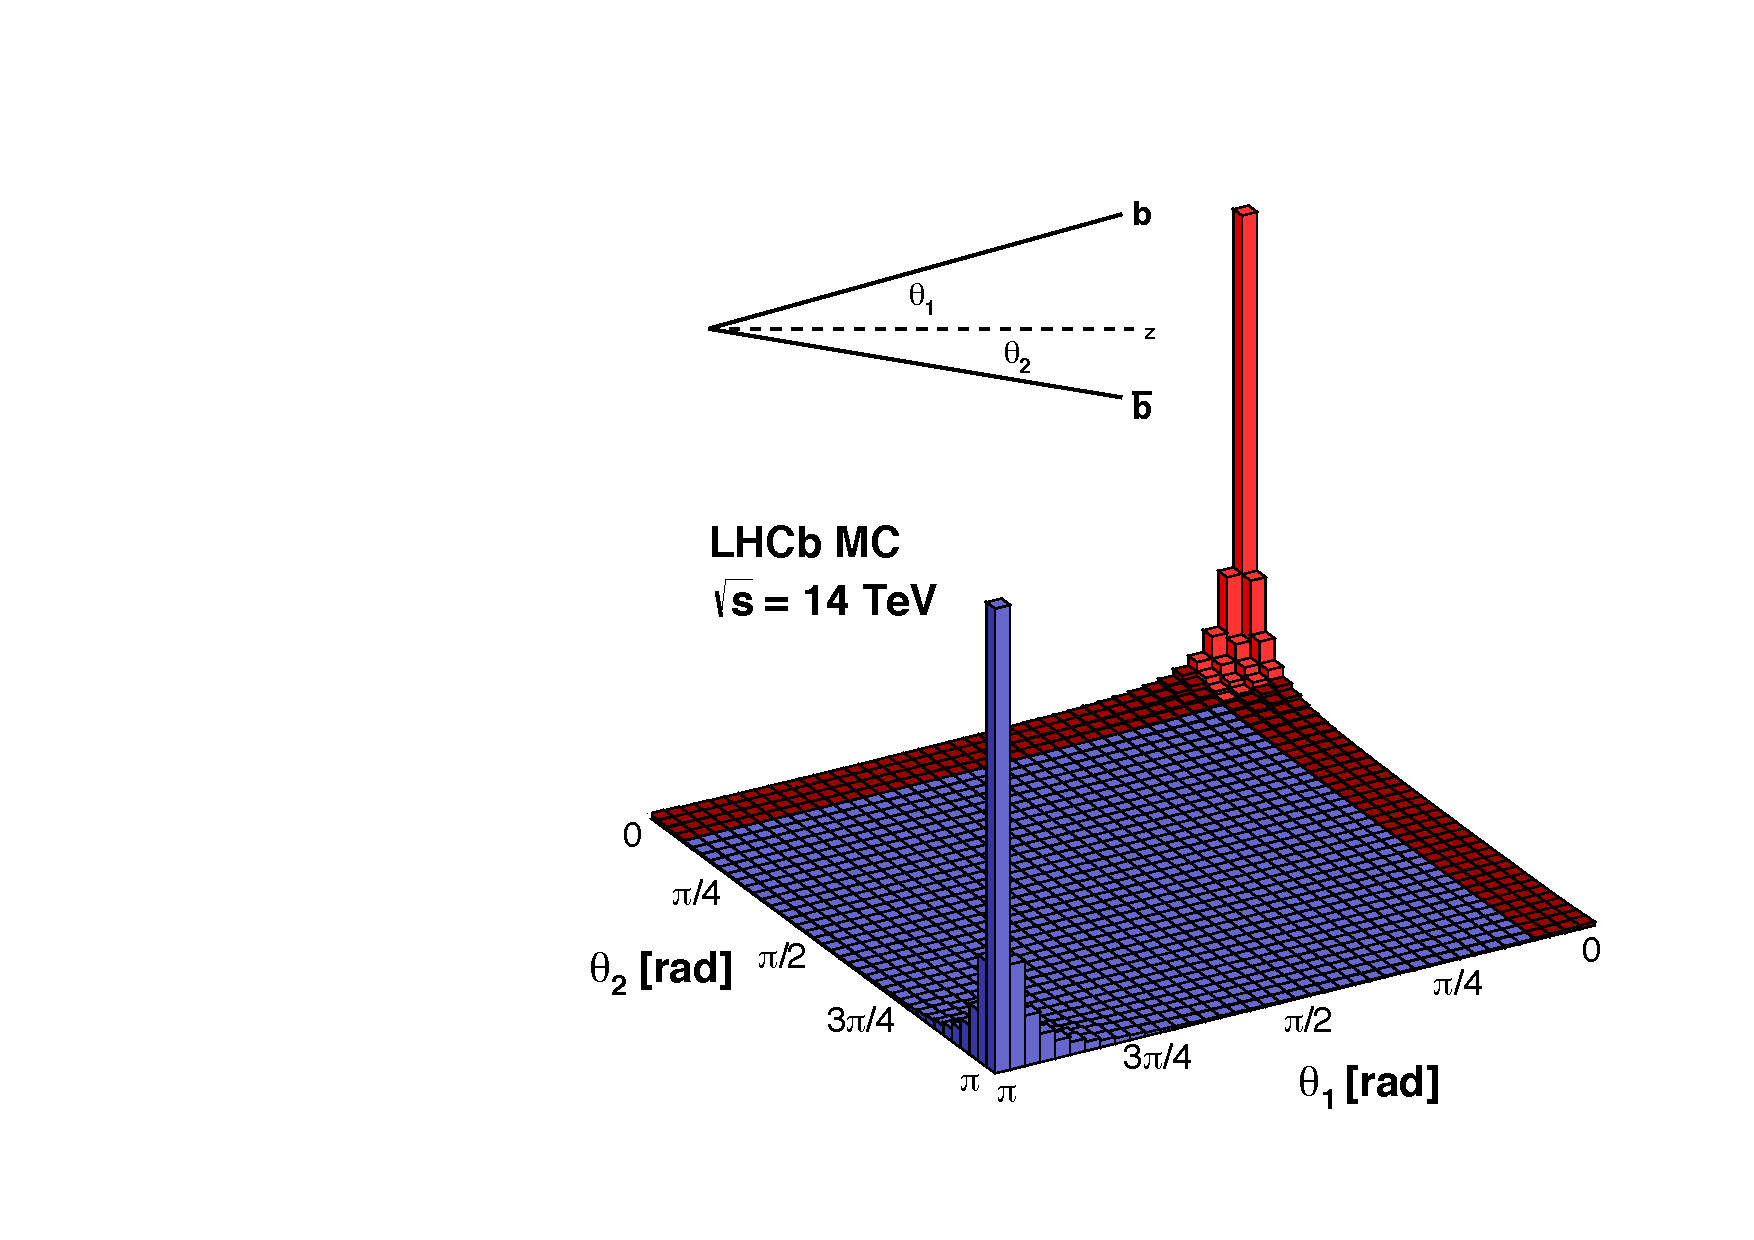
\includegraphics[width=\textwidth]{introduction/bbbar_production_angles}};
  \begin{scope}[x={(image.south east)}, y={(image.north west)}]
    % Grid to help find coordinates on the image
    % \draw[step=0.02, gray, very thin] (0, 0) grid (1, 1);
    % Box to cover axis labels
    \path[fill=white] (0.02, 0.16) rectangle (0.18, 0.22) node [pos=0.5] {\footnotesize$\theta_{1}$};
    \path[fill=white] (0.64, 0.06) rectangle (0.78, 0.12) node [pos=0.5] {\footnotesize$\theta_{2}$};
    % Box to cover angle definitions
    \path[fill=white] (0.14, 0.66) rectangle (0.54, 0.88);
    % Box to cover 'LHCb MC' label
    \path[fill=white] (0.14, 0.48) rectangle (0.36, 0.58);
  \end{scope}
\end{tikzpicture}

    \caption{$\Pbottom\APbottom$ production distribution}
    \label{fig:intro:lhcb:hf_production:bbbar_angles}
  \end{subfigure}
  \caption{%
    Feynman diagram of quark pair production via gluon-gluon fusion 
    (\subref*{fig:intro:lhcb:hf_production:gg_fusion}), and a simulation of the 
    angular distribution of \bbbar\ production at the \ac{LHC} at $\sqrt{s} = 
    \SI{13}{\TeV}$ (\subref*{fig:intro:lhcb:hf_production:bbbar_angles}).
  }
  \label{fig:intro:lhcb:hf_production}
\end{figure}

\begin{figure}
  \centering
  % Draw perpendicular markers at line intersections
% http://tex.stackexchange.com/a/21759/45857
\tikzset{
  right angle quadrant/.code={
    \pgfmathsetmacro\quadranta{{1,1,-1,-1}[#1-1]}     % Arrays for selecting quadrant
    \pgfmathsetmacro\quadrantb{{1,-1,-1,1}[#1-1]}},
  right angle quadrant=1, % Make sure it is set, even if not called explicitly
  right angle length/.code={\def\rightanglelength{#1}},   % Length of symbol
  right angle length=2ex, % Make sure it is set...
  right angle symbol/.style n args={3}{
    insert path={
      let \p0 = ($(#1)!(#3)!(#2)$) in     % Intersection
      let \p1 = ($(\p0)!\quadranta*\rightanglelength!(#3)$), % Point on base line
      \p2 = ($(\p0)!\quadrantb*\rightanglelength!(#2)$) in % Point on perpendicular line
      let \p3 = ($(\p1)+(\p2)-(\p0)$) in  % Corner point of symbol
      (\p1) -- (\p3) -- (\p2)
    }
  }
}
\begin{tikzpicture}[
  x=2cm,
  y=2cm,
  axis/.style={very thick,->,gray},
  beam/.style={very thick,->,gray},
  scale=1.5,
  thick
  ]
  % Origin
  \coordinate (O) at (0, 0);
  % B decay vertex
  \coordinate (Bvtx) at (1, 0.5);
  % Offset of muon arrows, with respect to Bvtx
  \coordinate(mumoffset) at (0.3, 0.4);
  \coordinate(mupoffset) at (0.6, -0.2);
  % Compute the coordinates of the ends of the muon lines
  \coordinate (mum) at ($(Bvtx) + (mumoffset)$);
  \coordinate (mup) at ($(Bvtx) + (mupoffset)$);

  % Coordinate axes
  \draw[axis] (-0.6, -0.5) -- +(0.2, 0) node [below] {$z$};
  \draw[axis] (-0.6, -0.5) -- +(0, 0.2) node [left] {$y$};

  \draw[beam] (-1.0, 0) -- (-0.1, 0) node [below, at start] {$p$};
  \draw[beam] (1.5, 0) -- (0.1, 0) node [below, at start] {$p$};

  % D meson
  \draw[dashed, color=gray, text=black] (O) -- (Bvtx) node [above, pos=0.5] {\PDz};
  % Negative child
  \draw[->] (Bvtx) -- (mum) node [above] {\PKminus};
  \draw[dotted] (Bvtx) -- ($(Bvtx) - 3*(mumoffset)$) node [name=mumend] {};
  % Positive child
  \draw[->] (Bvtx) -- (mup) node [below] {\Ppiplus};
  \draw[dotted] (Bvtx) -- ($(Bvtx) - 2*(mupoffset)$) node [name=mupend] {};

  % Primary vertex
  \node[star,star points=10,draw=orange!50,fill=orange!20,inner sep=0pt,minimum size=0.4cm] at (O) {};

  % Negative muon IP
  \draw[right angle length=1mm, right angle symbol={Bvtx}{mumend}{O}] ($(Bvtx)!(O)!(mumend)$) -- (O) node [pos=0.2, left] {$\text{IP}_{\PKminus}$};
  % Positive muon IP
  \draw[right angle length=1mm, right angle symbol={Bvtx}{mupend}{O}] ($(Bvtx)!(O)!(mupend)$) -- (O) node [midway, left] {$\text{IP}_{\Ppiplus}$};
\end{tikzpicture}

  \caption{%
    Illustration of vertexing, showing a \PDz meson decaying in flight to a 
    kaon and a pion.
    The kaon and pion are reconstructed as tracks, and then \PDz decay vertex 
    is inferred from the point of closest approach of the two tracks.
    The minimum transverse distance the tracks make when extrapolated back 
    towards the primary proton-proton vertex, the \acf{IP}, is shown.
  }
  \label{fig:intro:lhcb:vertexing}
\end{figure}

% The \ac{LHC} provides higher production rates of charm and beauty hadrons that 
% any previous collider, and \lhcb\ is the only dedicated heavy flavour 
% experiment at the \ac{LHC}.
% As such, its primary goal is to study the properties of charm and beauty 
% hadrons, exploiting the large amount of data that has been and continues to 
% made to make precise measurements.

% Unlike \atlas\ and \cms\, the \lhcb\ detector is searching for \ac{BSM} physics 
% primarily through indirect searches.
% The two principle methods in which this is done is through measuring 
% differences between matter and antimatter, and by measuring rare processes such 
% as the \BsTomumu decay.

\section{Detector}
\label{chap:intro:lhcb:detector}

When describing the detector, it is useful to define a common coordinate 
system.
Within the \lhcb\ experiment, it is customary to define a right-handed 
coordinate system, where the $z$-axis is aligned along the beam direction, 
increasing in the clockwise direction along the \ac{LHC} ring; the $y$-axis is 
aligned with gravity, increasing away from the Earth's surface; and the 
$x$-axis, defined as $x = y \times z$, is then increasing away from the centre 
of the accelerator.
In this section, and in all subsequent sections, this coordinate system will be 
used.

The detector is shown in \cref{fig:intro:lhcb:detector}.
How forward a process or a detector is is defined by the polar angle $\theta$, 
defined with respect to the beam, with $0 < \theta < \pi$.
A polar angle close to the extremes is considered forward, whilst values around 
$\sfrac{\pi}{2}$ are \emph{central}.
Another measure is the pseudorapidity
\begin{equation}
  \Eta = -\ln\left(\tan{\frac{\theta}{2}}\right).
  \label{eqn:intro:lhcb:pseudorapidity}
\end{equation}
The pseudorapidity is zero at $\sfrac{\pi}{2}$, and becomes infinite as 
$\theta$ tends to it extremes.
The general purpose \atlas\ and \cms\ detector are instrumented for particle 
tracking in the region $|\Eta| < 2.5$, whereas the \lhcb\ detector is 
instrumented in the region $2 < \Eta < 5$.

\begin{figure}
  \centering
  \begin{tikzpicture}
  % Use trim and crop to remove some of the white space around the image
  \node[anchor=south west, inner sep=0] (image) at (0, 0) {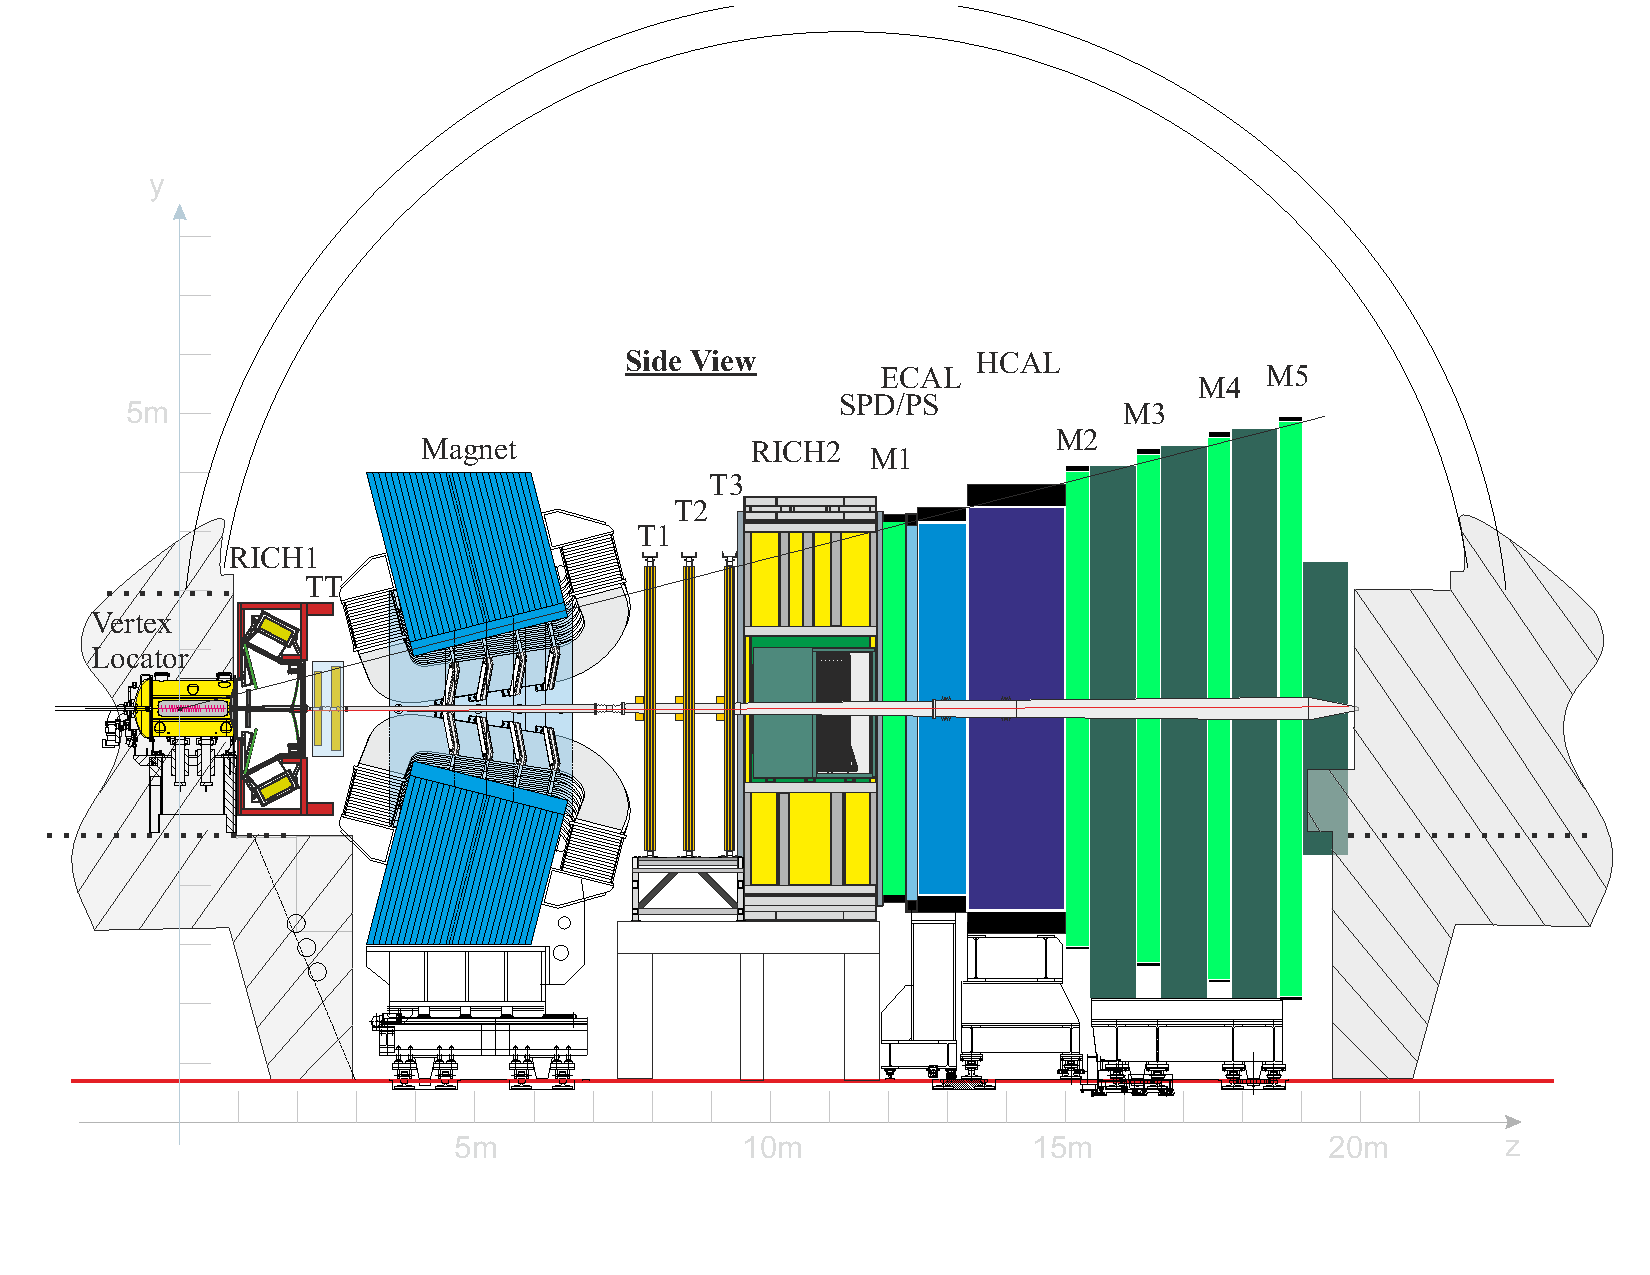
\includegraphics[width=\textwidth, trim={1cm 1.7cm 0.5cm 3cm}, clip]{introduction/lhcb_detector}};
  \begin{scope}[x={(image.south east)}, y={(image.north west)}]
    % Grid to help find coordinates on the image
    % \draw[step=0.02, gray, very thin] (0, 0) grid (1, 1);
    % Box to cover "Side View" label
    \path[fill=white] (0.36, 0.78) rectangle (0.46, 0.84);
  \end{scope}
\end{tikzpicture}

  \caption{%
    A schematic of the \lhcb\ detector.
    In this Figure, the $z$-axis, labelled, increases from left to right, the 
    $y$-axis, also labelled, increases from bottom to top, and the $x$-axis 
    increases into the page.
  }
  \label{fig:intro:lhcb:detector}
\end{figure}

\subsection{Tracking}
\label{chap:intro:lhcb:detector:tracking}

\subsection{Particle identification}
\label{chap:intro:lhcb:detector:pid}

\subsection{Event selection}
\label{chap:intro:lhcb:detector:trigger}

\subsection{Data flow}
\label{chap:intro:lhcb:detector:dataflow}
